\documentclass{homework}
\usepackage[light,math]{kurier}
\usepackage{graphicx}
\usepackage[T1]{fontenc}
\usepackage{hyperref}
\hypersetup{
    colorlinks=true,
    linkcolor=blue,
    filecolor=magenta,      
    urlcolor=cyan,
    }
\pagenumbering{goggle}
\SMALL{\author{TEJADHITH S}
\class{EE21BTECH11055}}
\title{\Large{Heart Rate and BP Measurement using PPG}}

\graphicspath{{./media/}}

\begin{document} \maketitle

\textbf{Abstract :}  Obtaining Heart rate and Blood Pressure using the Photoplethysmography(PPG) signal obtained from TCRT5000. Due to the systolic and diastolic cardiac cycle of heart results in change of blood volume in the finger which can be captured using PPG. The reflectance depends on the volume of blood flowing through the finger. So on filtering and processing the captured wave the heart rate and the blood pressure can be obtained.\\
 \\
 \textbf{Idea behind the Implementation :}\\
 \includegraphics[scale = 0.41]{Block1.png}
\textbf{Process/Steps Involved :}\\
\indent \textbf{1)} Biasing TCRT5000\\
\indent \textbf{2)} Passive High Pass Filter (HPF)\\
\indent \textbf{3)} Buffer\\
\indent \textbf{4)} Active Low Pass Filter (LPF)\\
\indent \textbf{5)} Inverting Amplifier and Rectifier\\
\indent \textbf{6)} Processing using Arduino (This can be done using Sampler-ADC-Encoder)\\
 \\
 \textbf{Biasing TCRT5000 :}\\
  \\
 TCRT5000 is setup of IR sensor cum PhotoTransistor that transmits IR (780nm - 1mm) EMR and the PhotoTransistor gives an Analog voltage output of transmitted/reflected IR EMR.\\
 TCRT5000 is biased according to Fig.1 (A). \\
 For Emitter (Diode) the maximum reverse voltage ($R_V$) that can be applied is 5V and the maximum forward current ($I_F$) can be 60mA.\\
 For the Detector (PhotoTransistor) the maximum emitter collector voltage ($V_{EC}$) applied can be 5V and maximum collector current ($I_C$) can be 100mA.\\
 Hence the input voltage given is (4-5)V and the obtained $I_F$ is 5mA. Where $I_C $ depends on incident light and 5V > $I_CR_1$ inorder to keep the transistor in the active region.\\
 \href{https://drive.google.com/file/d/1Nk3fOqGYrcH04Q41L5S5DGP_ae-Hyu3v/view?usp=sharing}{Link} to the biased TCRT5000 setup.\\
 The output from TCRT5000 can be observed in Fig.2 (A)\\
 \textcolor{red}{*(Note : Prolonged eye contact may cause damage to eye, So mobile camera can be used to check the working)}
\begin{center}
    \large{\texttt{Filtering and Amplification}}\\
\end{center}
\textbf{Passive High Pass Filter (HPF) :}\\
 \\
 Capacitor of 1$\mu$F  and Resistor of 330K$\Omega$ is used. Passive HPF can be circuited as in Fig.1 (B).\\
 So the Cut-Off frequency of HPF is,
 \[f_{HPF} = \frac{1}{2\pi RC} = \frac{1}{2\pi (0.33)} = 0.48HZ\]
 So this implies that the signal having frequency less than 0.48HZ will be filtered including the DC value arised due to the constant incident of light.\\
 Passive HPF is used in order to maintain high input impedance in order to not alter the output from transistor.\\
  \\
\textbf{Buffer :}\\
 \\
 The reason behind adding the buffer after passive HPF is to maintain high input impedance for active LPF.\\
 For Buffer 1st OPAMP of LM324N is used where the input is given to Non-Inverting terminal and Inverting/Output terminals are connected.\\
 The output observed after Passive HPF + Buffer is Fig.2 (B).\\
 \\
\textbf{Active Low Pass Filter :}\\
Resistor of (10K$\Omega$ and 1K$\Omega$), Capacitor of 4.7$\mu$F and 2nd OPAMP of LM324N is used. The active LPF is circuited as in Fig.1 (B). The cut-off frequency of LPF is,
\[f_{LPF} = \frac{1}{2\pi RC} = \frac{1}{2\pi (0.047)} = 3.39HZ\]
So this implies that the signal with frequency higher than 3.39HZ will be filtered (High frequency components).\\
And Active LPF amplifies the input by 10x as A = 10K$\Omega$/1K$\Omega$ (Inverting).\\
The output observed after Active LPF is Fig.2 (C).\\
 \\
\textbf{As the Heart rate lies in the range of (60-190) bpm which is (1-3.16)HZ, Hence the above mentioned $f_c$ is chosen.}\\
\textbf{Amplification :}\\
 \\
Resistor of (22K$\Omega$ and 1K$\Omega$) and 3rd OPAMP of LM324N is used. Inverting Amplifier can be circuited as in Fig.1 (D).\\
The Gain of the inverting Amplifier is,
\[A = \frac{R_7}{R_6} = \frac{22K}{1K} = 22\]
Hence the input is getting amplified by 22x.\\
The output observed after Amplification is Fig.2 (D).\\
\textbf{\href{https://drive.google.com/file/d/1NpnrK1EjaQGCwMMTEyrYlUoaqjVxqCX3/view?usp=sharing}{Link} to the Filter and Amplification Setup.}
\begin{figure}[h]
    \includegraphics[scale = 0.38]{Circuit1.png}
    \caption{}
\end{figure}\\
\fbox{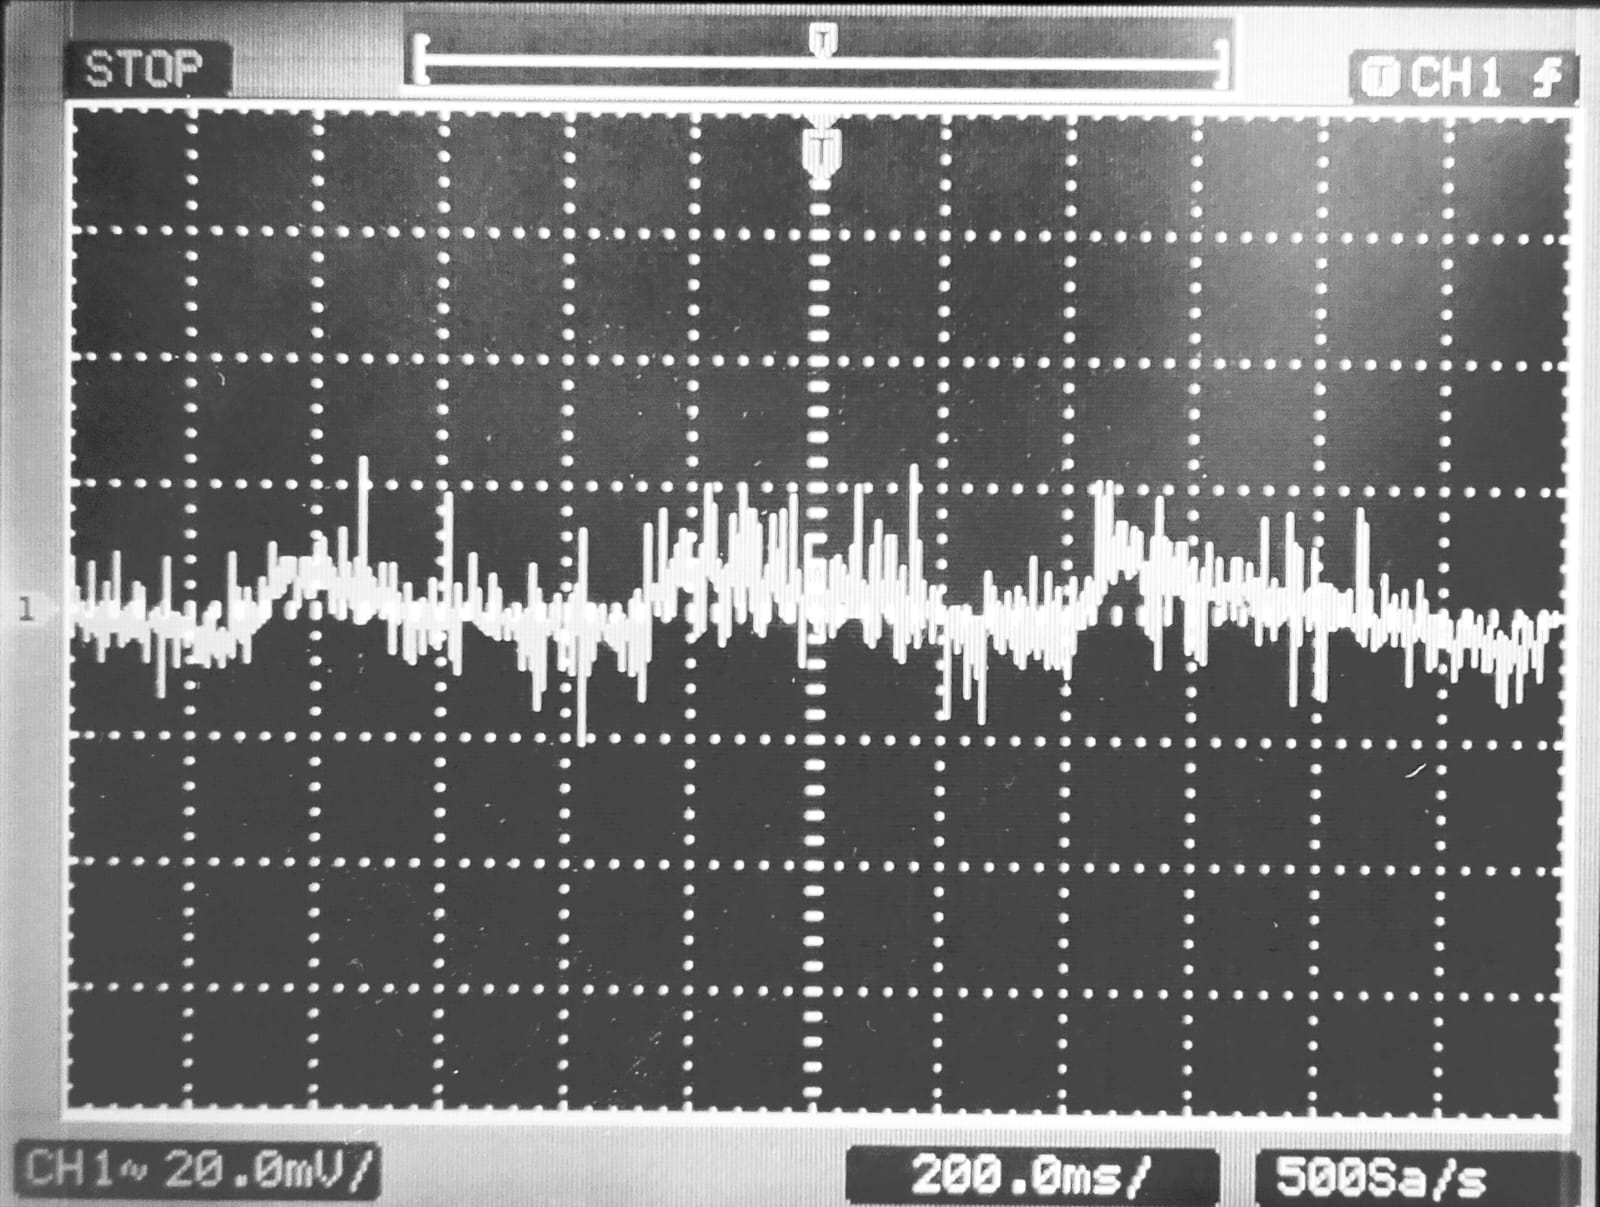
\includegraphics[scale = 0.079]{Fig2A.png}}
\fbox{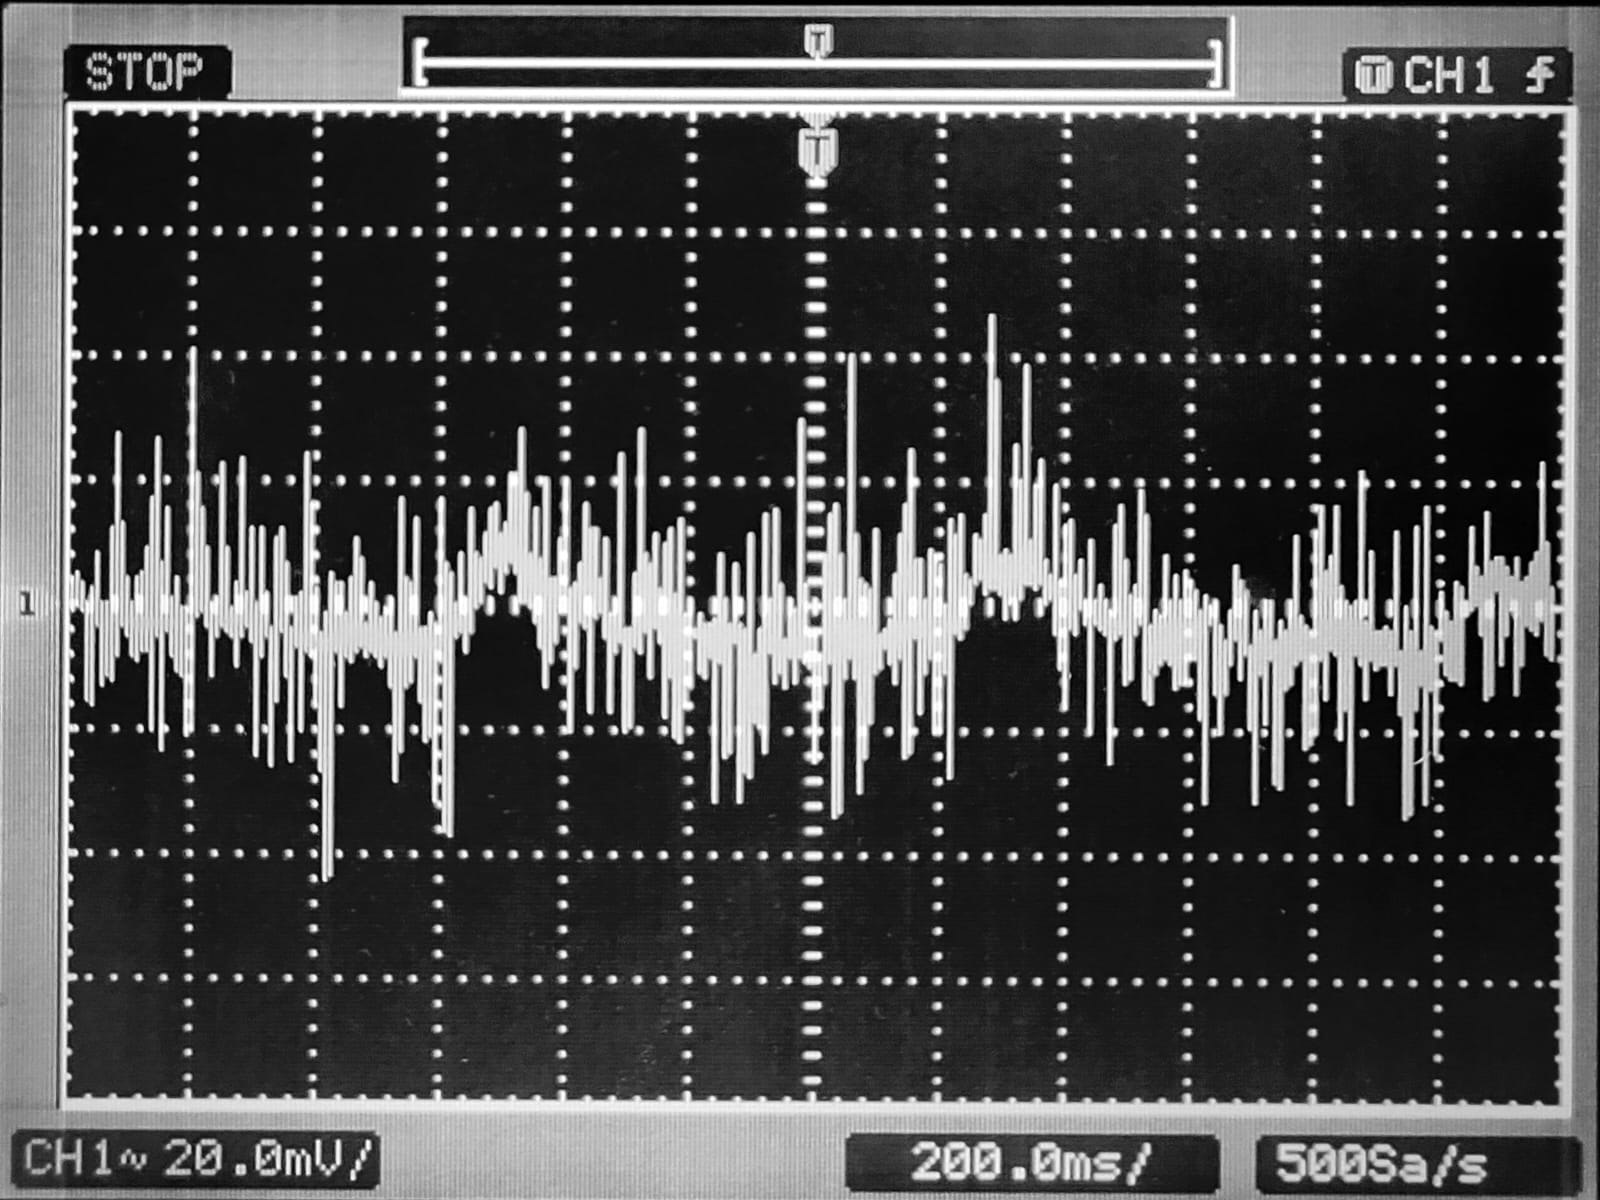
\includegraphics[scale = 0.079]{Fig2B.png}}
\fbox{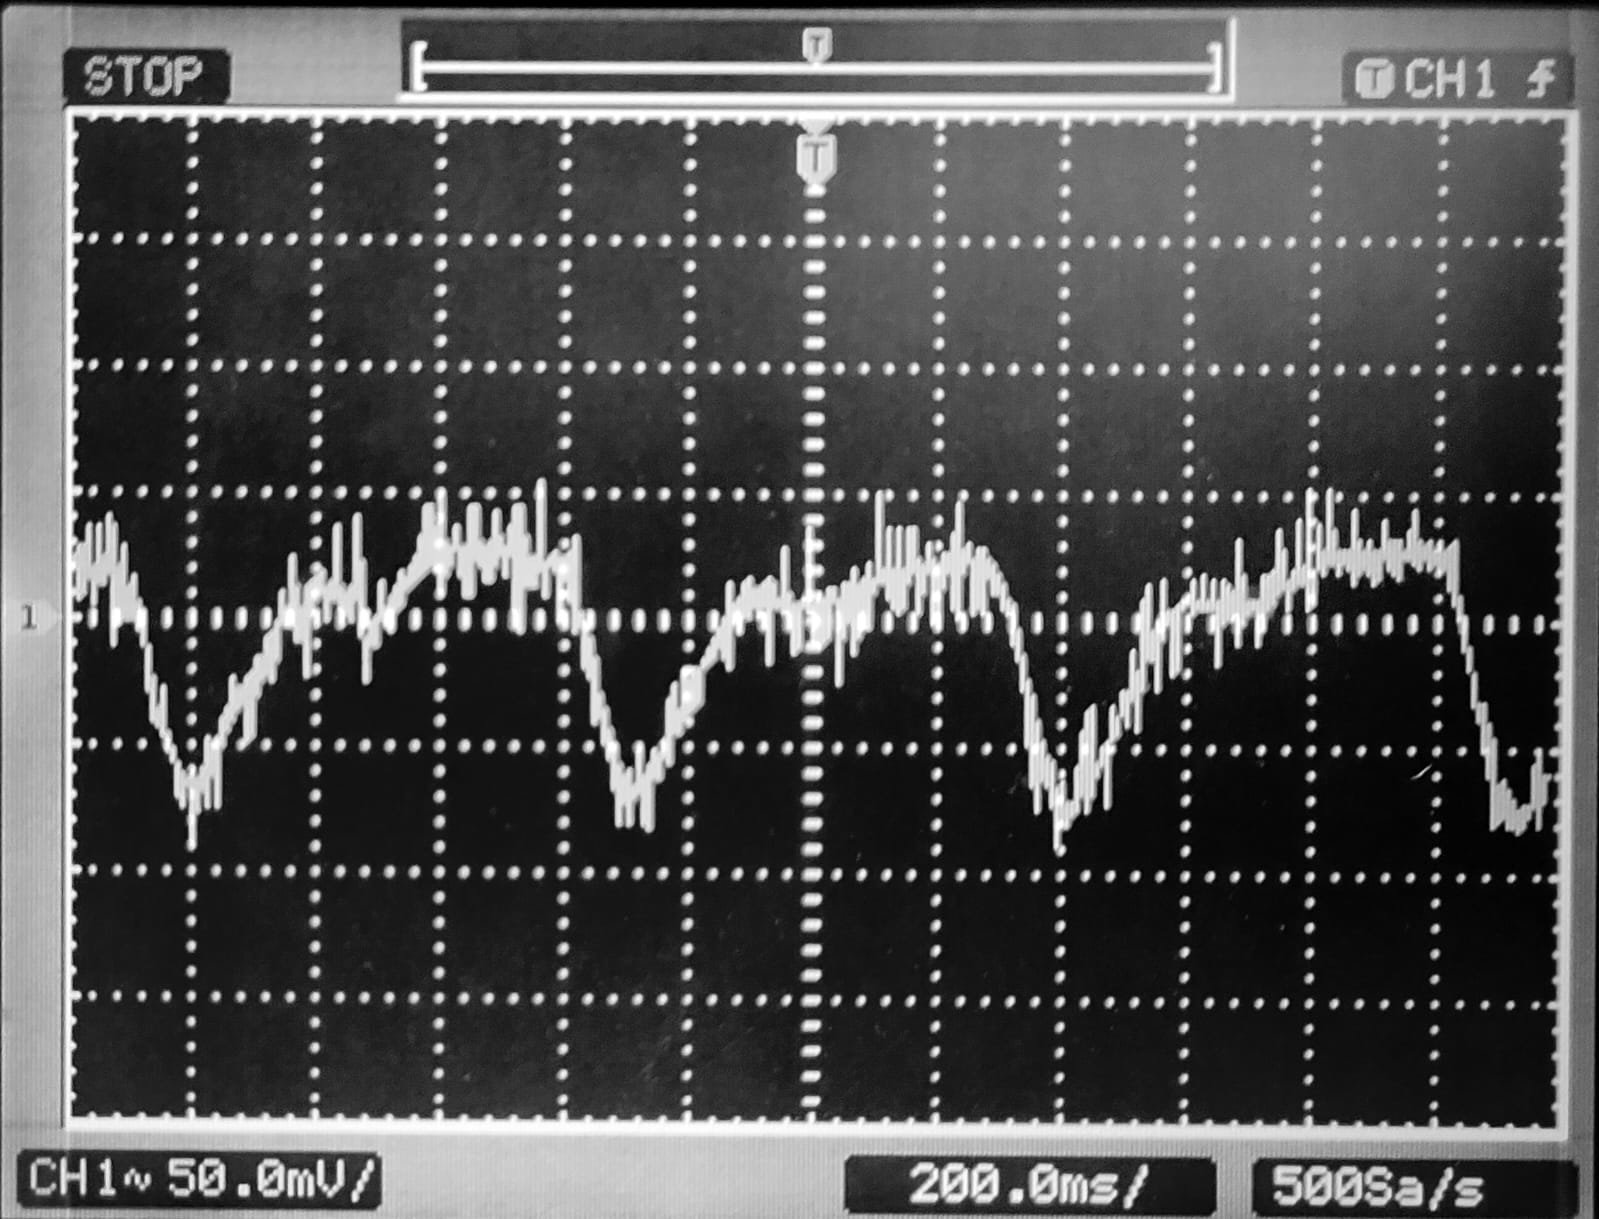
\includegraphics[scale = 0.079]{Fig2C.png}}
\fbox{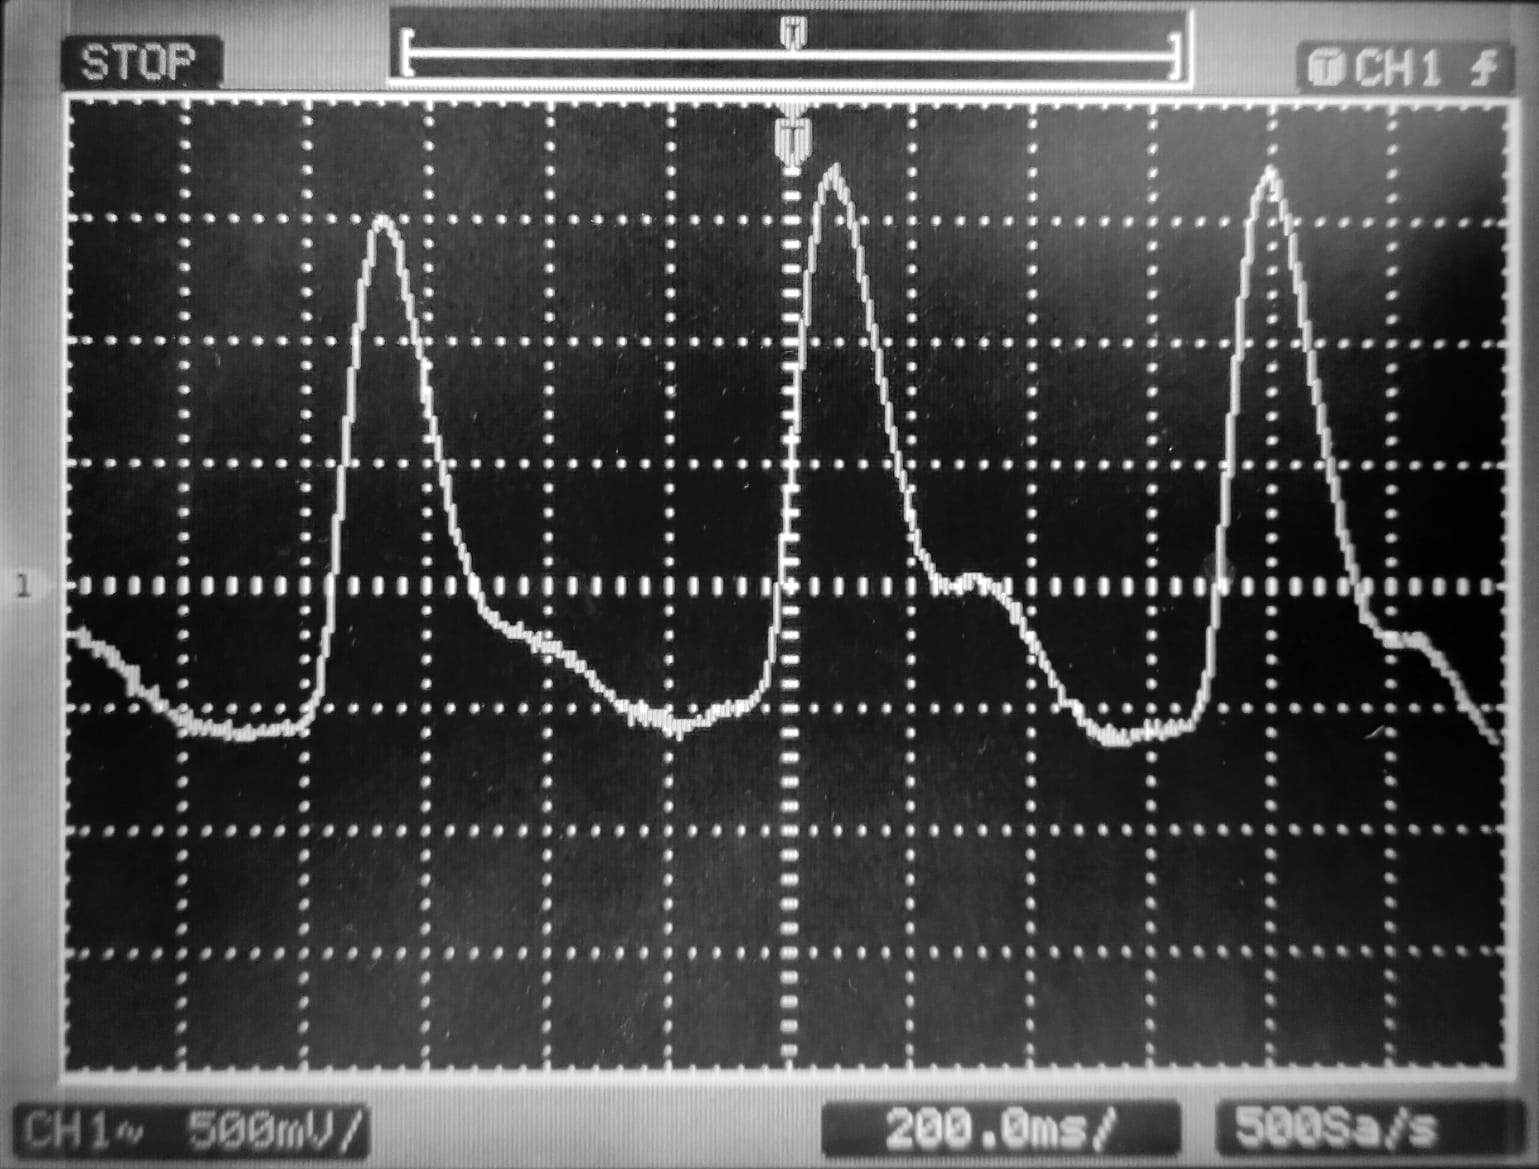
\includegraphics[scale = 0.079]{Fig2D.png}}
\indent\ \ \ \ \ \text{Figure.2 (A)}\indent\ \ \ \ \ \ \ \ \ \ \ \ \ \ \ \ \ \ \ \ \text{Figure.2 (B)}\indent\  \ \ \ \ \ \ \ \ \ \ \ \ \ \ \ \text{Figure.2 (C)}\indent\ \ \ \ \ \ \ \ \ \ \ \  \ \ \  \text{Figure.2 (D)} \\
\begin{center}
    \large{\texttt{Processing using Arduino}}\\
\end{center}
The signal received from the Amplifier has to be sampled using ADC and FFT(Fast Fourier Transform) has to be performed in order to obtain the peak. The accuracy of the FFT depends on the Sampling frequency and the duration of sampling. The sampling frequency is taken to be 16HZ (Default Sampling Frequency of Arduino) which means in 1 second 16 samples (input) is taken from the signal. And coded such that sampling is done for 16s.
\[ \text{Heart Rate} = \frac{60xSampling FrequencyxPeak}{No. of Samples}\]
And Blood Pressure can be calculated using the same setup using the following formula,
\begin{align*}
    \text{Systolic BP} = 184.3 - 1.32xHR + 0.0848xT_d\\
\text{Diastolic BP} = 55.96 - 0.02912xHR + 0.023xT_d
\end{align*}
Where, $T_d = HR(\text{in ms}) - Timedelay$, Timedelay is taken as the time difference between Maximum frequency and Minimum frequency.\\
The output from amplifier is given to an Analog pin (A0) of Arduino and the ground of Arduino is connected to ground of the circuit.\\
The Arduino is programmed accordingly using certain libraries. \href{https://github.com/TEJADHITH/bpm_bp_measurement/blob/main/using_arduino.ino}{Here} is the code used in the Arduino in order to measure the Heart Rate and Blood Pressure.\\
\textbf{Conclusion :}\\
Here is the \href{https://drive.google.com/file/d/1NNSSBI55vghyBbqjyvGRnKfu3BkBh4d0/view?usp=share_link}{Link} to the video of measurement of Heart Rate and Blood Pressure (Systolic and Diastolic). And here is the \href{https://drive.google.com/file/d/1Xyi8ULlUVJIfOv-L8Huq1mbdpNMJOM5w/view?usp=share_link}{Link} to screenshot of serial monitor of Arduino while measuring BP and Heart Rate.
\begin{center}
    \large{\texttt{Processing using Discrete Components}}\\
\end{center}
\textbf{Sampler :}\\
A MOSFET (N7000) and Capacitor of Capacitance 2.2pF is used to sample the signals. The sampler digitizes the given analog signal and holds the signals for ADC. The sampler can be circuited as in Fig.3 (A). The output observed after passing through sampler is Fig.4\\
 \\
\textbf{ADC (Analog to Digital Converter) :}\\
In order to design ADC, 2 LM324N (7 OPAMP) and 8 resistors of resistance 2K$\Omega$ is used. ADC can be circuited as in Fig.3 (B).\\
So it's a 3 bit ADC which has 8 outputs. It works such that for $V_{in}>V^-$(Inverting Terminal) then the output from the respective OPAMP is $V_{CC}$ which is 5V.\\
Hence Arduino is programmed with logic to encode the input from 8 digital pins (8 bit to 3 bit Encoder).\\
\href{https://github.com/TEJADHITH/bpm_bp_measurement/blob/main/using_components.ino}{Here} is the code for the logic behind the encoder.\\
\textbf{\href{https://drive.google.com/file/d/1Nff5NuQ25jewDKzhwKrg-UZLwyj3tnhR/view?usp=sharing}{Link} to the Sampler and ADC Setup.}
\begin{figure}[h]
    \centering
    \includegraphics[scale = 0.35]{Circuit2.png}
\end{figure}
 \\
  \\
   \\
    \\
    \\
    \\
\indent \ \ \ \ \ \ \ \ \ \ \ \ \ \ \ \ \ \ \  \ \ \ \ \ \ \ \ \ \ \ \ \ \ \ \ \ \   \ \ \ \  \ \ \ \ \ \ \  \ \ \ \ \ \ \ \ \ \ \ \ Figure 3\\
\begin{center}
    \fbox{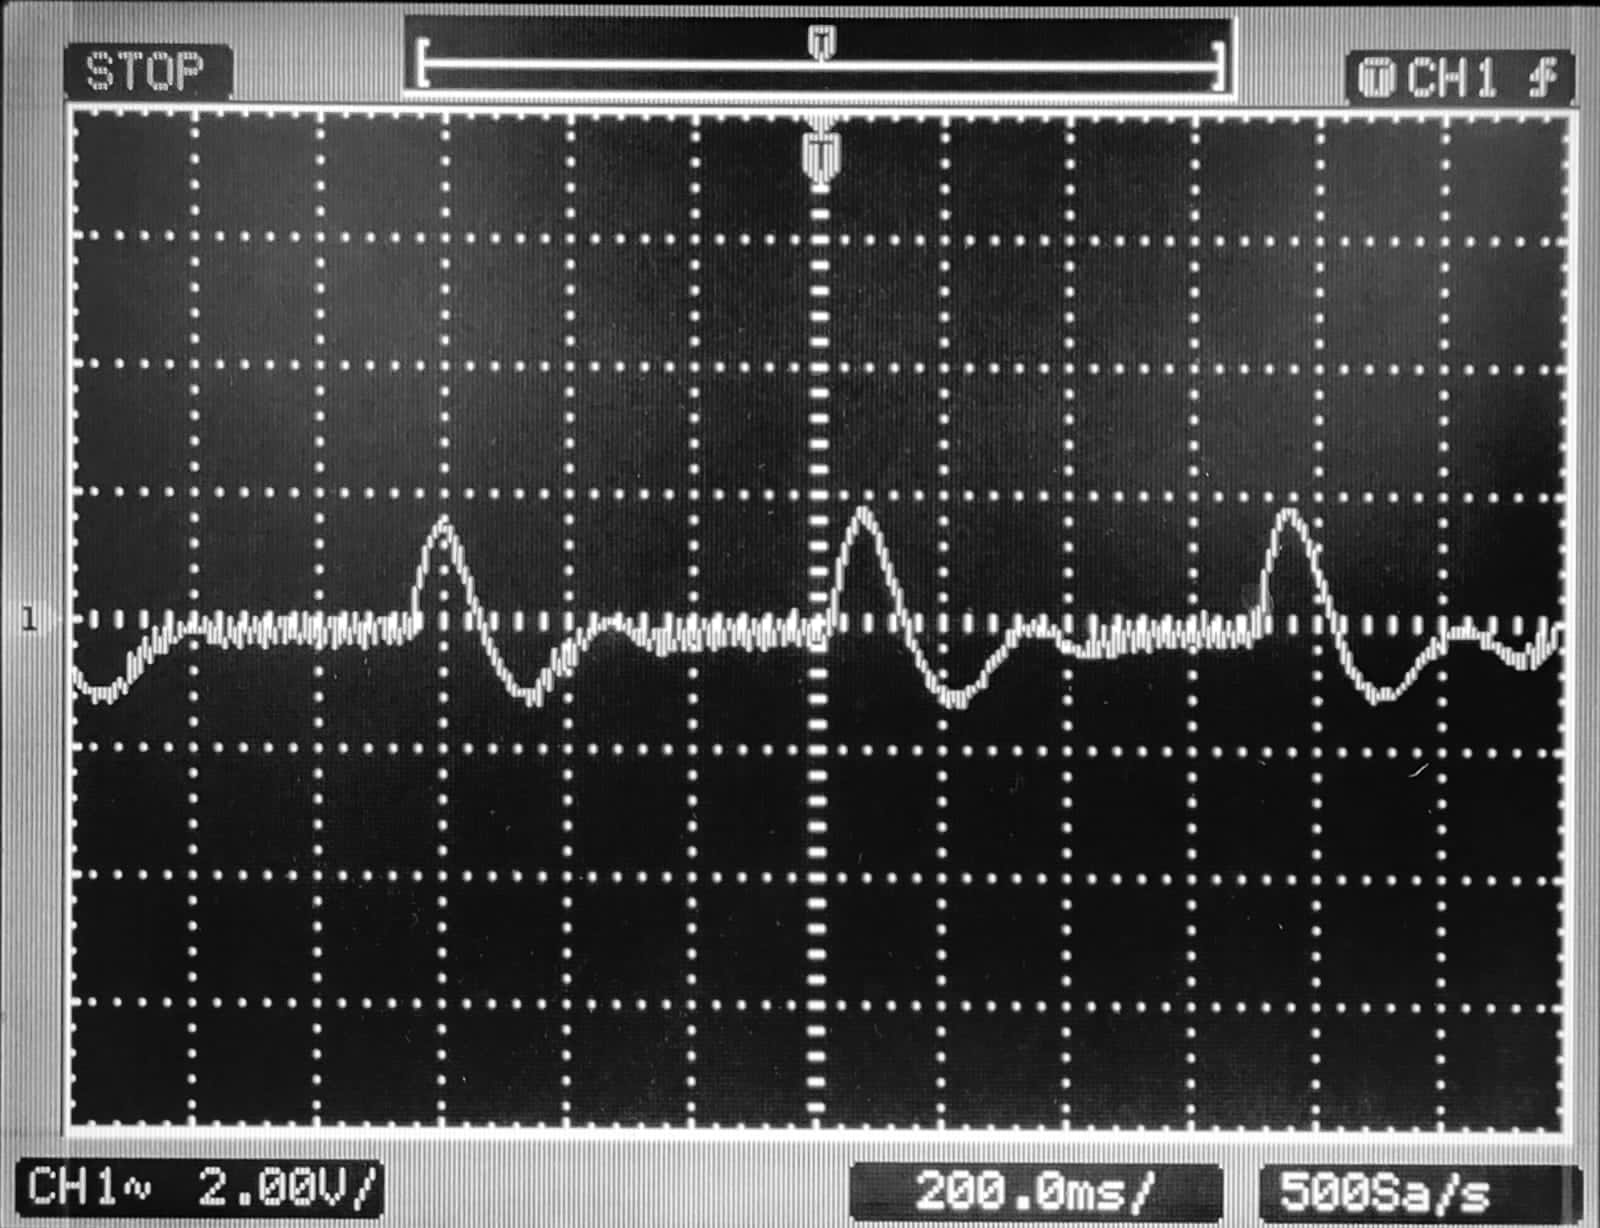
\includegraphics[scale = 0.11]{Fig4.png}}\\
\end{center}
\indent \ \ \ \ \ \ \ \  \ \ \ \ \  \ \  \ \ \ \ \ \ \ \ \ \ \ \  \ \ \ \ \ \ \ \ \ \ \ \ \ \ \ \ \ \ \ \ \ \  \ \ \ \ \ \ \ \ \ \ \ \ Figure 4 \\
 \\
\textbf{Conclusion :}\\
The values obatained after encoding is plotted using serial plotter. Then the FFT of the obatained wave is calculated. The difference between the peaks are calculated and the frequency is calculated then the heart rate is obtained by multiplying the frequncy by 60.\\
Here is the \href{https://drive.google.com/file/d/1NPStH7hU0MxG5iE_yXVHSs0OpeId46x4/view?usp=share_link}{Link} for the video of obtaining the digital signal from ADC and encoding it and \href{https://1drv.ms/x/s!AuQYwSGEkrzP3CZkBo6J1Lu3KujK?e=yTcLPL}{Link} for the excel sheet obtained after encoding.
\begin{center}
    \texttt{Supporting Materials}
\end{center}
1) \href{https://drive.google.com/drive/folders/1NKXPOUdBulDcIGyHvjaXw_hG5qdx01pC?usp=sharing}{Drive Link Containing all the Videos and Pictures}\\
2) \href{https://github.com/TEJADHITH/bpm_bp_measurement}{Github Repository}\\
3) \href{https://microcontrollerslab.com/lm324-op-amp-pinout-datasheet-applications-features-datasheet/}{LM324N Pin Configuration}
\begin{center}
    \texttt{References}
\end{center}
1) http://www.ee.iitb.ac.in/~stallur/wp-content/uploads/2017/02/Heart-Rate-Measurement-using-PPG1.pdf\\
2) https://github.com/udiboy1209/heart-rate-monitor
\end{document}